\subsection{General View}
    \noindent \begin{minipage}{0.5\textwidth}
        \vspace{1cm}
        \fbox{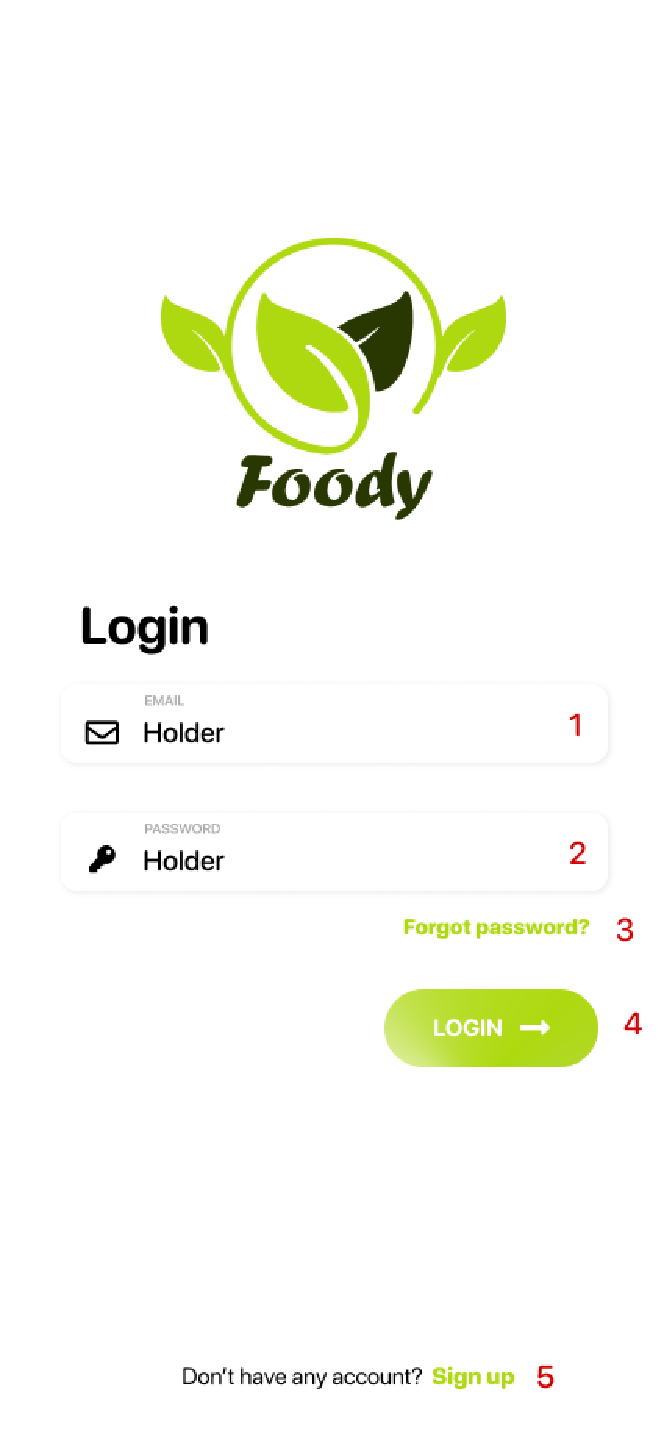
\includegraphics[width=\textwidth]{images/ui/Login.pdf}}
        \captionof{figure}{Trang đăng nhập}
        \label{fig:nature}
    \end{minipage}
    \hspace{0.05\textwidth}
    \begin{minipage}{0.45\textwidth}
        \begin{tblr}{
            width=1\linewidth,
            hlines, 
            vlines,
            colspec={X[1]X[2]X[7]},
            columns = {valign = m, },
            column{1} = {halign = c},
            row{1} = {halign = c, valign = m, bg = lightgray, fg = black},
            }
            {\textbf{\#}} & \textbf{Type} & {\textbf{Mô tả}} \\
            1 & Input & Người dùng nhập email\\
            2 & Input &  Người dùng nhập password\\
            3 & Link & Chuyển đến trang quên mật khẩu\\
            4 & Button & Xác nhận đăng nhập \newline
                         Hệ thống kiểm tra, nếu đúng, chuyển sang trang chủ\\
            5 & Link & Chuyển sang trang đăng ký \\
        \end{tblr}
    \end{minipage}
    
    \newpage
    \noindent \begin{minipage}{0.5\textwidth}
        \vspace{1cm}
        \fbox{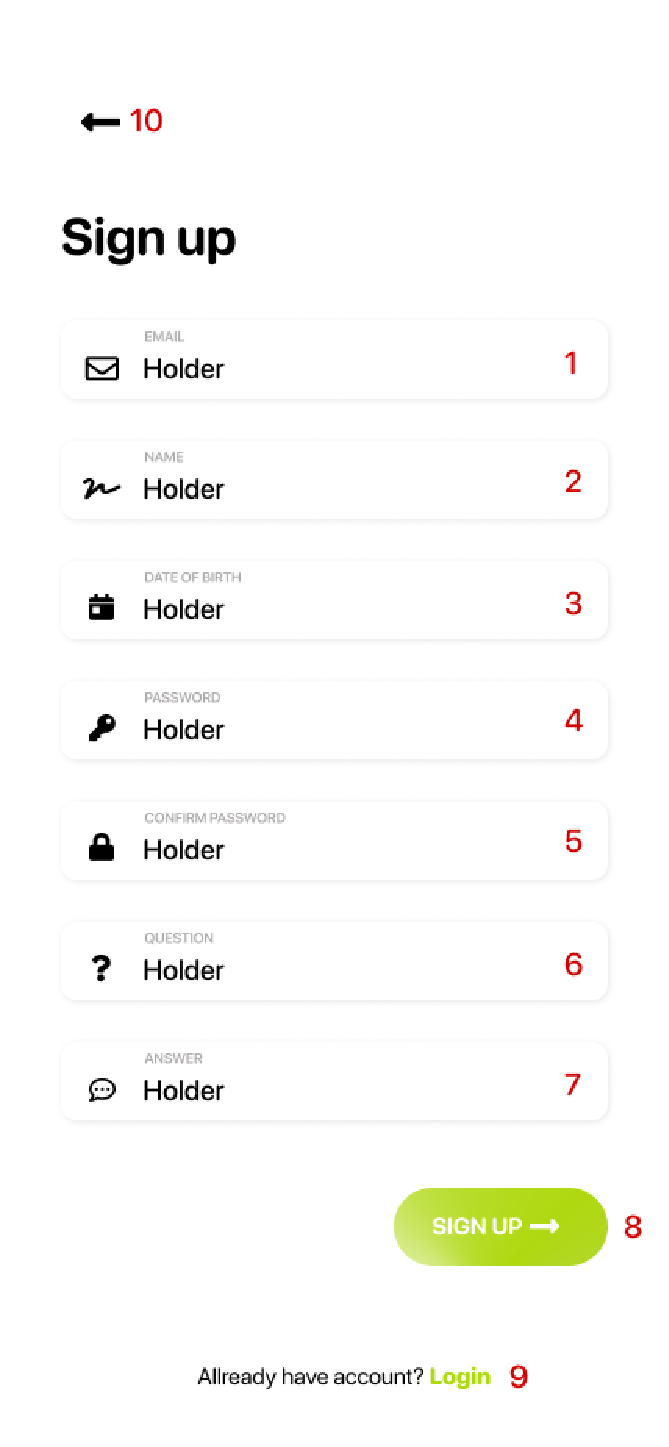
\includegraphics[width=\textwidth]{images/ui/Sign up.pdf}}
        \captionof{figure}{Trang đăng ký tài khoản}
        \label{fig:nature}
    \end{minipage}
    \hspace{0.05\textwidth}
    \begin{minipage}{0.45\textwidth}
        \begin{tblr}{
            width=1\linewidth,
            hlines, 
            vlines,
            colspec={X[1]X[2]X[7]},
            columns = {valign = m, },
            column{1} = {halign = c},
            row{1} = {halign = c, valign = m, bg = lightgray, fg = black},
            }
            {\textbf{\#}} & \textbf{Type} & {\textbf{Mô tả}} \\
            1 & Input & Người dùng nhập email\\
            2 & Input &  Người dùng nhập tên\\
            3 & Input &  Người dùng nhập ngày sinh\\
            4 & Input &  Người dùng nhập password\\
            5 & Input &  Người dùng xác nhận mật khẩu\\
            6 & Input &  Người dùng nhập câu hỏi bí mật\\
            7 & Input &  Người dùng nhập câu trả lời\\
            8 & Button & Xác nhận đăng ký \newline
                         Hệ thống kiểm tra, nếu thỏa, chuyển sang trang đăng nhập\\
            9 & Link & Chuyển sang trang đăng nhập\\
            10 & Button & Quay lại trang đăng nhập\\
        \end{tblr}
    \end{minipage}
    
    \newpage
    \noindent \begin{minipage}{0.5\textwidth}
        \vspace{1cm}
        \fbox{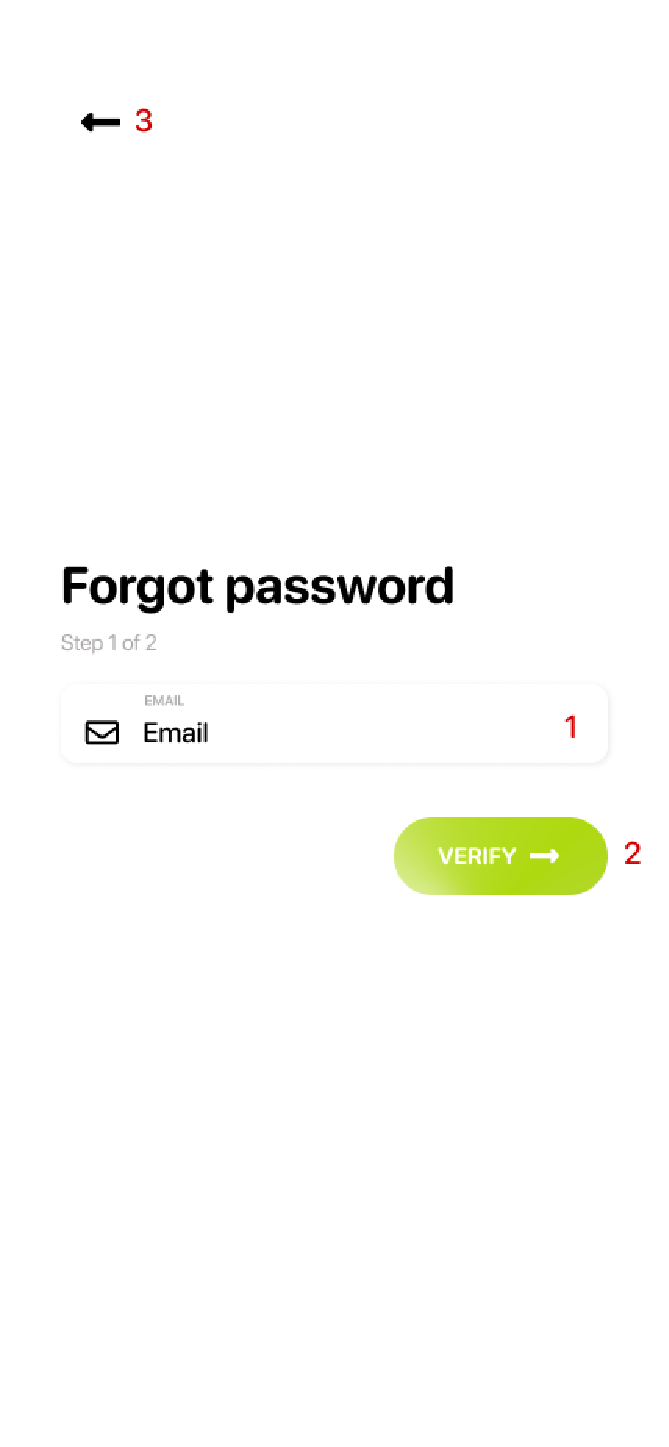
\includegraphics[width=\textwidth]{images/ui/Forgot password-1.pdf}}
        \captionof{figure}{Trang đăng quên mật khẩu (Bước 1)}
        \label{fig:nature}
    \end{minipage}
    \hspace{0.05\textwidth}
    \begin{minipage}{0.45\textwidth}
        \begin{tblr}{
            width=1\linewidth,
            hlines, 
            vlines,
            colspec={X[1]X[2]X[7]},
            columns = {valign = m, },
            column{1} = {halign = c},
            row{1} = {halign = c, valign = m, bg = lightgray, fg = black},
            }
            {\textbf{\#}} & \textbf{Type} & {\textbf{Mô tả}} \\
            1 & Input & Người dùng nhập email\\
            2 & Button & Xác nhận email \newline
                         Hệ thống kiểm tra, nếu thỏa, chuyển sang bước 2\\
            3 & Button & Quay lại trang đăng nhập\\
        \end{tblr}
    \end{minipage}
    
    \newpage
    \noindent \begin{minipage}{0.5\textwidth}
        \vspace{1cm}
        \fbox{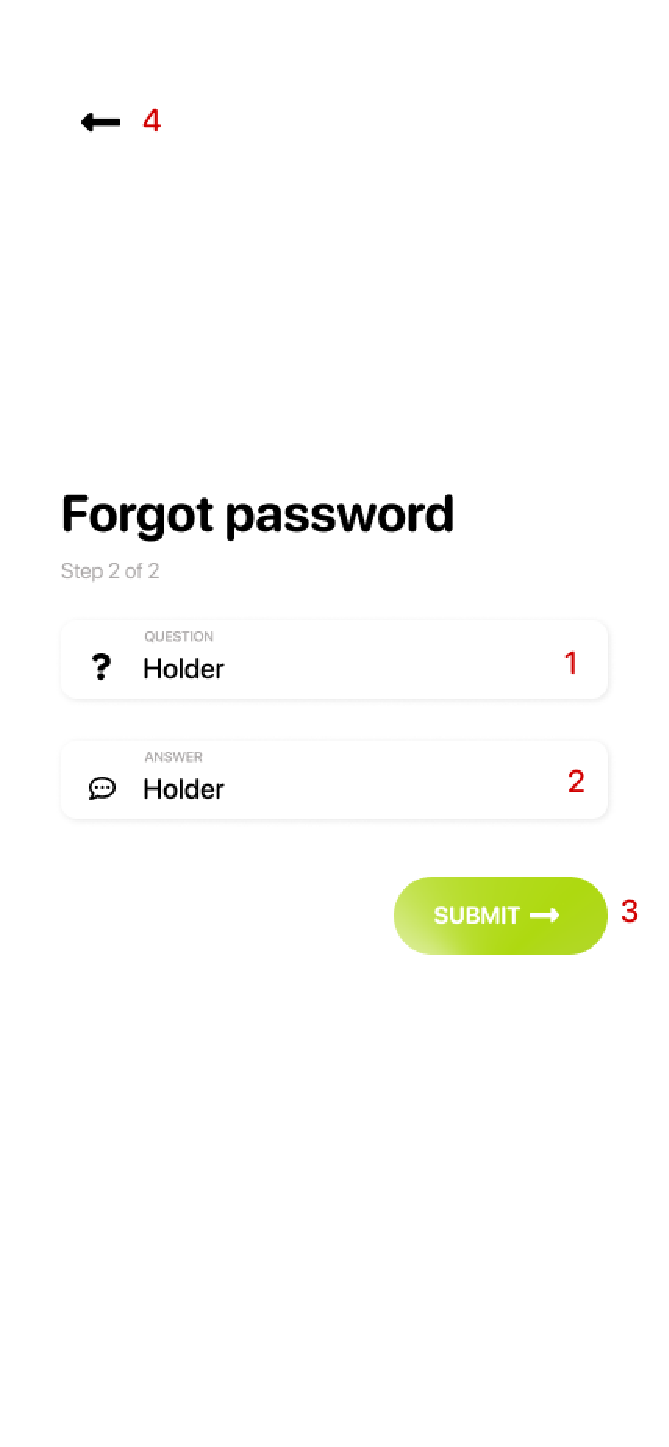
\includegraphics[width=\textwidth]{images/ui/Forgot password-2.pdf}}
        \captionof{figure}{Trang đăng quên mật khẩu (Bước 2)}
        \label{fig:nature}
    \end{minipage}
    \hspace{0.05\textwidth}
    \begin{minipage}{0.45\textwidth}
        \begin{tblr}{
            width=1\linewidth,
            hlines, 
            vlines,
            colspec={X[1]X[2]X[7]},
            columns = {valign = m, },
            column{1} = {halign = c},
            row{1} = {halign = c, valign = m, bg = lightgray, fg = black},
            }
            {\textbf{\#}} & \textbf{Type} & {\textbf{Mô tả}} \\
            1 & Input &  Người dùng nhập câu hỏi bí mật\\
            2 & Input &  Người dùng nhập câu trả lời\\
            3 & Button & Xác nhận đăng ký \newline
                         Hệ thống kiểm tra, nếu thỏa, mật khẩu sẽ được hiện lên màn hình\\
            4 & Button & Quay lại bước 1\\
        \end{tblr}
    \end{minipage}
    
    \newpage
    \noindent \begin{minipage}{0.5\textwidth}
        \vspace{1cm}
        \fbox{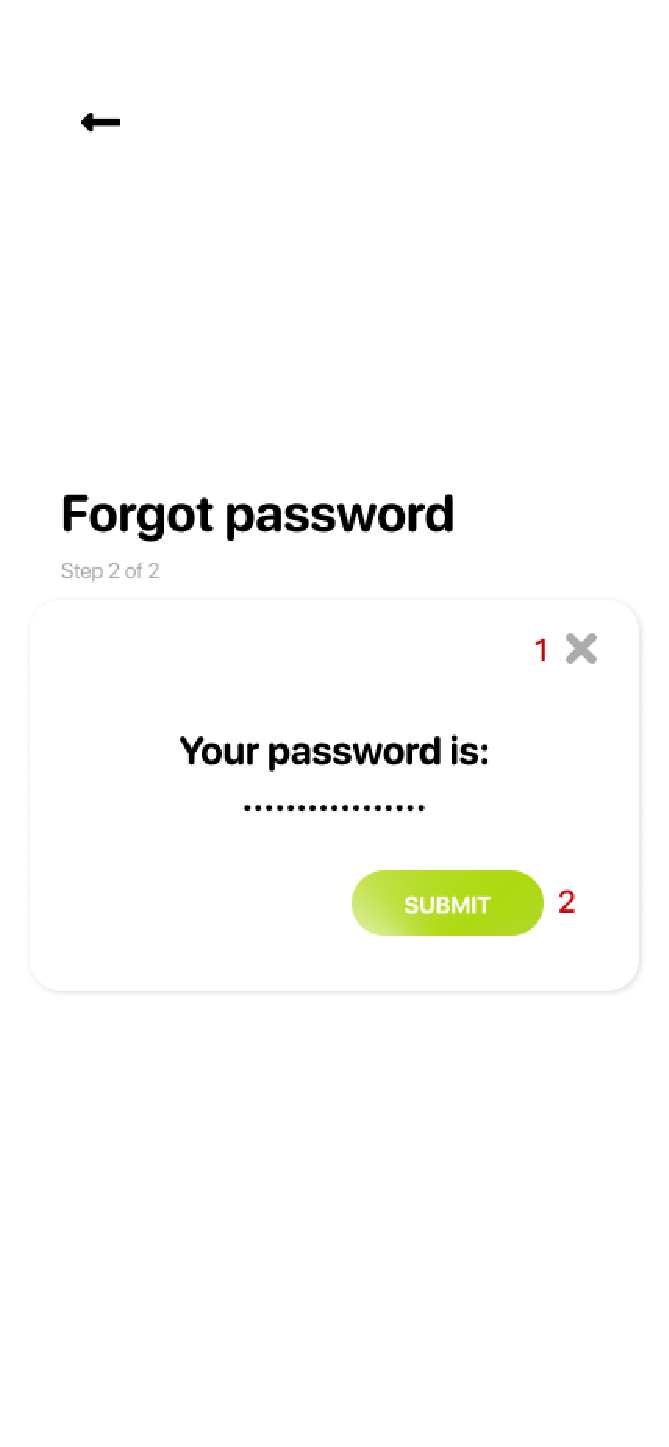
\includegraphics[width=\textwidth]{images/ui/Forgot password-3.pdf}}
        \captionof{figure}{Trang đăng quên mật khẩu (Hiện mật khẩu)}
        \label{fig:nature}
    \end{minipage}
    \hspace{0.05\textwidth}
    \begin{minipage}{0.45\textwidth}
        \begin{tblr}{
            width=1\linewidth,
            hlines, 
            vlines,
            colspec={X[1]X[2]X[7]},
            columns = {valign = m, },
            column{1} = {halign = c},
            row{1} = {halign = c, valign = m, bg = lightgray, fg = black},
            }
            {\textbf{\#}} & \textbf{Type} & {\textbf{Mô tả}} \\
            1 & Button & Đóng bảng thông báo\\
            2 & Button & Đóng bảng thông báo và quay lại trang đăng nhập\\
        \end{tblr}
    \end{minipage}
    
    \newpage
    \noindent \begin{minipage}{0.5\textwidth}
        \vspace{1cm}
        \fbox{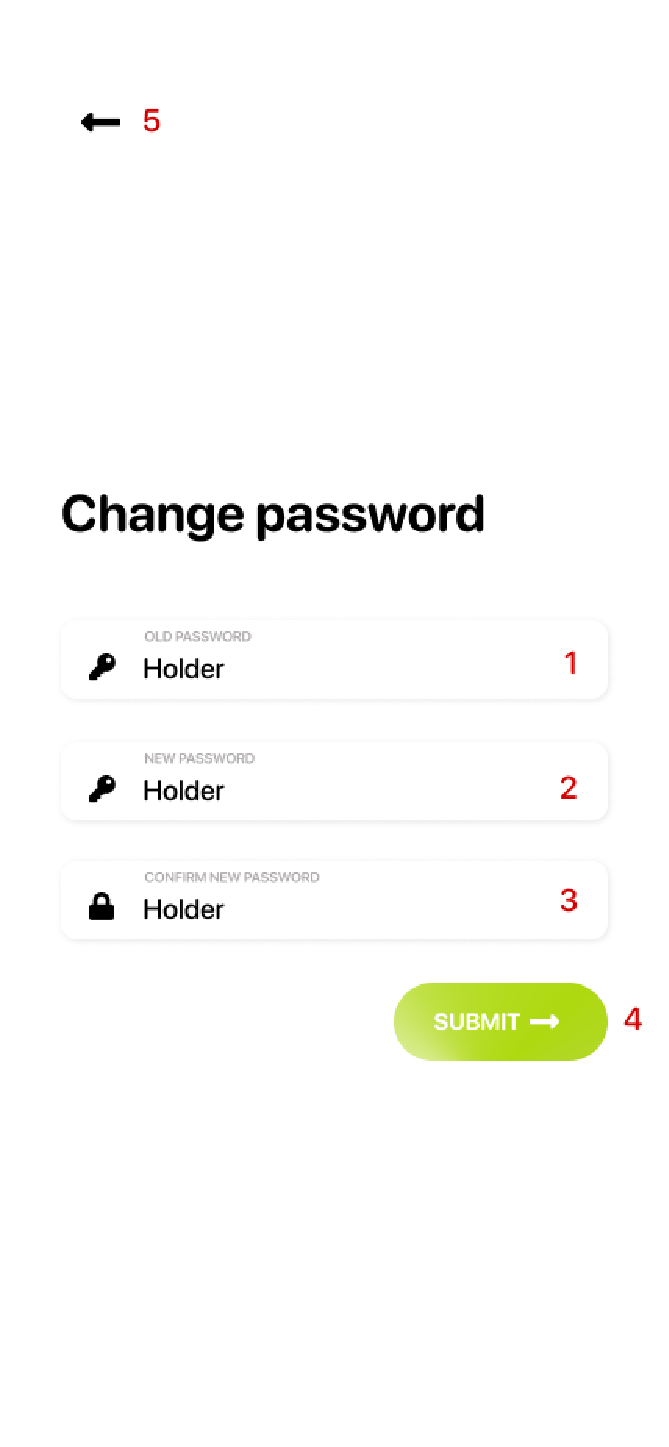
\includegraphics[width=\textwidth]{images/ui/Change password-1.pdf}}
        \captionof{figure}{Trang đổi mật khẩu}
        \label{fig:nature}
    \end{minipage}
    \hspace{0.05\textwidth}
    \begin{minipage}{0.45\textwidth}
        \begin{tblr}{
            width=1\linewidth,
            hlines, 
            vlines,
            colspec={X[1]X[2]X[7]},
            columns = {valign = m, },
            column{1} = {halign = c},
            row{1} = {halign = c, valign = m, bg = lightgray, fg = black},
            }
            {\textbf{\#}} & \textbf{Type} & {\textbf{Mô tả}} \\
            1 & Input & Người dùng nhập mật khẩu cũ\\
            2 & Input & Người dùng nhập mật khẩu mới\\
            3 & Input & Người dùng xác nhận khẩu mới\\
            4 & Button & Xác nhận đổi mật khẩu, nếu thành công, hiện thông báo\\
        \end{tblr}
    \end{minipage}
    
    \newpage
    \noindent \begin{minipage}{0.5\textwidth}
        \vspace{1cm}
        \fbox{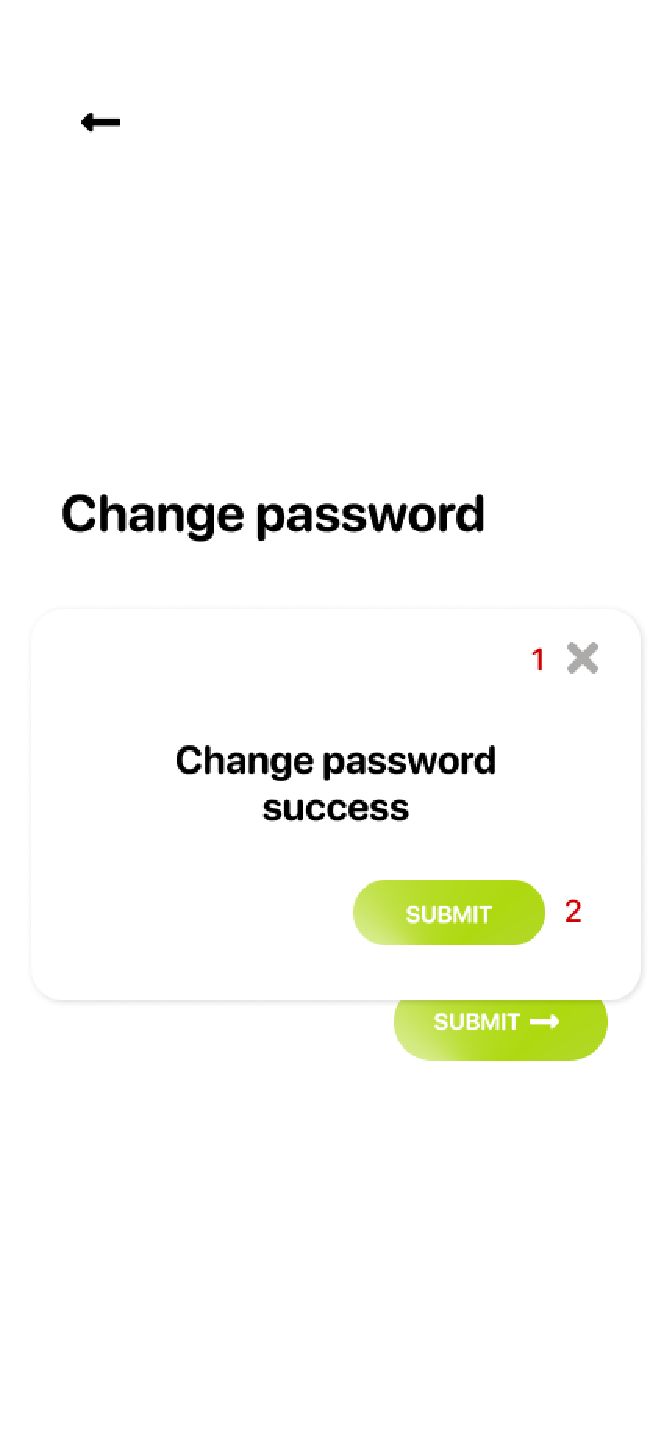
\includegraphics[width=\textwidth]{images/ui/Change password-2.pdf}}
        \captionof{figure}{Trang đổi mật khẩu (hiện thông báo)}
        \label{fig:nature}
    \end{minipage}
    \hspace{0.05\textwidth}
    \begin{minipage}{0.45\textwidth}
        \begin{tblr}{
            width=1\linewidth,
            hlines, 
            vlines,
            colspec={X[1]X[2]X[7]},
            columns = {valign = m, },
            column{1} = {halign = c},
            row{1} = {halign = c, valign = m, bg = lightgray, fg = black},
            }
            {\textbf{\#}} & \textbf{Type} & {\textbf{Mô tả}} \\
            1 & Button & Đóng bảng thông báo\\
            2 & Button & Đóng bảng thông báo và quay lại trang đăng nhập\\
        \end{tblr}
    \end{minipage}
